\Th $\forall n \geqslant 4 \forall k \leqslant \frac{n}{4} \forall s : 2 \leqslant ln \frac{sk}{n} \leqslant k$: $\exists M: \tau (M) \geqslant \frac{1}{32} \cdot  \frac{n}{k} ln \frac{sk}{n}$

Будем пользоваться неравенством $[x] \geqslant \frac{x}{2}$.

\Proof Пусть $m = [\frac{1}{2} ln \frac{sk}{n}] \geqslant 1$. Рассмотрим $N_1, \dots, N_{C_{2m}^m} \subset \{ 1, 2, \dots, 2m\} \subset \{1, 2, \dots, n\} = R_n$, где $N_i$ - все возможные m-элементные подмножества, $|N_i| = m$. 

$\tau (\{N_1, \dots, N_{C_{2m}^m}\}) = m + 1$, потому что если взять любое m-эл. мн-во найдётся обратное к нему. 

$q = [\frac{2k}{m}]; \frac{k}{m} \geqslant \frac{2k}{ln \frac{sk}{n}} \geqslant 2 \Rightarrow q \geqslant 4$

Разобьем на такие множества размера $2m$.
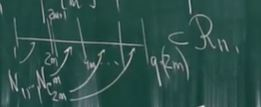
\includegraphics[]{images/est2.JPG}

В каждое разбиение размера $2m$ запихиваем совокупность выше ($N_1, \dots, N_{C_{2m}^{m}}$).

Рассмотрим множества $L_1 = N_1^1 \cup N_1^2 \cup \dots N_1^q$; $\dots$ $L_{C_{2m}^{m}} = N_{C_{2m}^{m}}^1 \cup N_{C_{2m}^{m}}^2 \cup \dots N_{C_{2m}^{m}}^q$; $ \forall i |L_i| = q\cdot m = [\frac{2k}{m}] \cdot m \geqslant \frac{k}{m} \cdot m = k$

$\tau (\{L_1, \dots, L_{C_{2m}^{m}}) = m + 1$ (очевидно, т.к. объединения одинаковые, сохраняется предыдущий результат для $\tau$).

$C_{2m}^m < 2^{2m} \leqslant 2^{ln \frac{sk}{n}} < e^{ln \frac{sk}{n}} = \frac{sk}{n}$

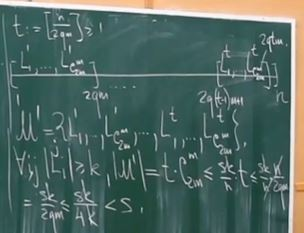
\includegraphics[]{images/est3.JPG}

$\tau(M') = t(m+1) > tm \geqslant \frac{n}{4qm} m \geqslant \frac{nm}{8k} \geqslant \frac{1}{32} \frac{n}{k} ln \frac{sk}{n}$. Но если какое-то из множеств мощности больше, чем k, то просто удалим из него любые элементы (соп от этого не уменьшится). $\tau(M'') \geqslant \tau(M')$
\EndProof